%===============================================================================
% $Id: ifacconf.tex 19 2011-10-27 09:32:13Z jpuente $  
% Template for IFAC meeting papers
% Copyright (c) 2007-2008 International Federation of Automatic Control
%===============================================================================
\documentclass{elsarticle}
\usepackage{textcomp}
\usepackage[utf8x]{inputenc} 
\usepackage[T1]{fontenc}
\usepackage[brazil,portuges]{babel}
\bibliographystyle{elsarticle-harv}
\biboptions{authoryear}
\usepackage{lipsum}
\usepackage{caption} 
\usepackage{hhline} % para usar linha dupla na tabela
\usepackage{tabularx} % para igualar colunas
\usepackage{dcolumn} % para efetuar alinhamento

\usepackage[table,xcdraw]{xcolor}
\usepackage{graphicx}      % include this line if your document contains figures
\usepackage{indentfirst}
\usepackage{subfigure}
%===============================================================================
\begin{document}
\begin{frontmatter}

\title{Classification of the maturation levels of the Caline IPA-06 tomato through image processing} 
% Title, preferably not more than 10 words.

\author[First]{Diego.V} 
\author[Second]{Arnon XX.}
\author[Room]{Airton XX.}
\author[Third]{Tales XX.}
\author[Fifth]{Igor S.}


\address[First]{Universidade Federal de Sergipe, SE 49100-000 BR (e-mail: vidal.center@academico.ufs.br);}
\address[Second]{Universidade Federal de Sergipe, SE 49100-000 BR (e-mail: xxxxxx@xxxxx.com);}
\address[Room]{Universidade Federal de Sergipe, SE 49100-000 BR (e-mail:  xxxxxx@xxxxx.com);}
\address[Third]{Universidade Federal de Sergipe, SE 49100-000 BR (e-mail:  xxxxxx@xxxxx.com;}
\address[Fifth]{Universidade Federal de Sergipe, SE 49100-000 BR (e-mail:  xxxxxx@xxxxx.com).}


\begin{abstract}% Abstract of not more than 250 words.
Parâmetros fisiológicos como acidez, massa, e cor destacam-se como indicadores de maturação em tomates, porém exigem tempo e trabalho para medições.A possibilidade de usar a Processamento de imagens (PDI) associados aos sistemas de previsão desses
variáveis fisiológicas podem auxiliar na predição e manutenção da qualidade dos tomates após a colheita de forma mais rápida e não invasiva. Com este objetivo, foi realizado um experimento com tomates Caline IPA-06, delineados experimentalmente ao acaso utilizando cinco repetições durante cinco períodos de maturação (0, 3, 6, 9 e 12 dias). Foram avaliadas as variáveis: Acidez titulável, PH, Sólidos solúveis, Massa fresca e Cor. Para analise da atividade biológica através do PDI foi utilizado o método biospeckle laser através das técnicas de Momento de Inercia (MI) e Diferença Generalizada (DG), todas sobre filtragem com aberturas de janelas através do filtro Wavelet. 
Nos resultados obtidos através deste modelo de simulação em PDI, quando comparado com demais evidenciaram existir correlação com a diminuição na taxa da atividade biológica e a perda de massa fresca. As amostras apresentaram mudanças significativas, para sólidos solúveis, cor  e PH mas estas não demostraram correlação com o comportamento do biospeckle.
\end{abstract}
\begin{keyword}
Lycopersicon esculentum, Processamento de imagens, Biospeckle Laser.
\end{keyword}
\end{frontmatter}

\section{Introduction}

Este trabalho baseia-se na ocorrência de um fenômeno óptico conhecido na física como speckle dinâmico, tendo sua nomenclatura, sofrido alterações à medida que se descobriu novas aplicações para o mesmo, atualmente conhecido como biospeckle dinâmico. Uma dessas alterações atribui ao fenômeno a denominação biospeckle, sendo esta, adotada preferencialmente quando o fenômeno ocorre em consequência de alguma atividade biológica 
\citet{Rodrigues2007} entre outros autores, descreve o fenômeno da seguinte forma:
\begin{citacao} %recuo a 4cm citação direta
“O biospeckle ou speckle dinâmico é um fenômeno óptico de interferência que ocorre quando há incidência de luz coerente em materiais, cujas superfícies sejam opticamente rugosas e que possuem algum tipo de atividade."
\end{citacao}

O embasamento teórico e experimental aponta no sentido de que é possível identificar a frequência de biospeckle que sofre interferência da variação do comportamento do fruto em relação a mudanças durante a maturação \cite{Zdunek2014}. Em materiais biológicos, os níveis de atividades estão diretamente relacionados com a viabilidade celular, troca de gases, respiração, atividade microbiana e atividade de água (aw). Este tipo de análise é importante, pois, se aplicada na fase de pós-colheita, pode abrir caminho para diversas aplicações como o desenvolvimento de sensores para avaliação qualidade do fruto, bem como a identificação do tempo de prateleira que o fruto pode suportar. 
 Por esta razão, o fenômeno tem sido estudado como uma potencial ferramenta na análise de qualidade e viabilidade de diversos materiais biológicos, como a viabilidade de sêmem \cite{Henrique2007a}, viabilidade de sementes arbóreas \cite{Aparecida2011}, mapeamento de atividade de água residuais \cite{Viana2017}. 
Na Engenharia Agrícola os esforços no emprego da técnica têm se concentrado na busca por métodos rápidos, objetivos e não destrutivos para a avaliação de materiais biológicos, sobretudo na área de pós-colheita, sendo os principais estudos relacionados à, mapeamento de áreas com atividades distintas \cite{Rabelo2005}, avaliação da qualidade do grão de café \cite{Viana2017}, do teor de água e identificação de espécies de fungos \cite{Hadian2008a}. 
As principais técnicas empregadas na análise do fenômeno são baseadas na variação temporal dos dados com estatísticas de primeira e segunda ordem, tais como a História Temporal do Speckle (STS) e as Matrizes de Ocorrências Modificadas (MOC), permitindo tanto a criação de mapas de atividades, empregando técnicas tais como as Diferenças Generalizadas (DG) e o Método de Fuji, como a quantificação do fenômeno, empregando a técnica conhecida como Momento de Inércia (MI) ou Módulo de Dispersão de Intensidades (MDI). 
Até o momento, as propostas de utilização do biospeckle laser têm ficado restritas ao laboratório, uma vez que diversos fatores como a vibração ambiental e ruídos externos, podem interferir nas medições, exigindo que as mesmas sejam feitas em ambiente controlado. No entanto, estudos recentes envolvendo a análise de bandas de frequências do biospeckle laser \cite{Lama2016}, demonstram ser possível utilizar as Transformadas de Wavelets (TW) e as Transformadas de Fourier (TF) e Transformada de Fourier Janelada (TFJ), para isolar frequências do padrão de atividade do biospeckle, permitindo assim, estabelecer uma correlação entre determinadas frequências e os elementos físicos e/ou biológicos que as perturbaram.

Sabe-se que os avanços mais notáveis no campo de máquinas agrícolas dos últimos tempos têm se dado no campo da agricultura de precisão, que busca o controle de forma precisa dos parâmetros e variáveis responsáveis por influenciar toda cadeia produtiva, como por exemplo, o tempo de prateleira dos frutos. Para atingir este propósito, sensores são instalados nas máquinas, permitindo que os dados referentes à qualidade seja comparados com outros fatores, o que possibilita um controle mais efetivo, preciso e econômico dos parâmetros que elevam o valor econômico. Por outro lado, Um dos fatores que está intimamente relacionado com a produtividade agrícola, diz respeito à controle e conservação pós-colheira. A atividade fisiológica do fruto e responsável durabilidade deste sendo determinante o entendimento e o controle das ações fisiológicas que possam diminuir a qualidade e o tempo do fruto. No entanto, os métodos usuais atualmente são deletérios,e probabilísticos para produção em grande escala, além de trazer prejuízo pelo descarte das amostras, levam um certo tempo para avaliar a durabilidade e o estado atual de maturação. O embasamento teórico associado ao fenômeno biospeckle laser, permite supor que as atividades de maturação do tomate podem ser quantificada de forma indireta, e suas perturbações nas frequências de atividade podem ser estudadas e classificadas com técnicas de análise de frequência.
Diante dos fatos apresentados, este projeto visa propor o estudo e modelamento da atividade de maturação do tomate IPA6 corroborando com métodos utilizados atualmente. Este conhecimento será importante, pois no futuro, poderá ser usado para o desenvolvimento de sensores que permitirão indicar de forma indireta, a qualidade do fruto, bem como seu tempo de prateleira, contribuindo para a agregação de valor no mercado comercial de hortaliças. 



\section{Materials and methods}

\subsection{Análises físico-químicas} 

%\newpage


\subsection{Delineamento Experimental}

\subsubsection{Methodology for image capture}
Com o Lazer HeNe 632nm incidindo nas amostras de solo \ref{fig:laser}, foram coletadas imagens através de método direto que consistia dos vídeos  direto da câmera através de um cabo AVI e uma conectado em uma placa de vídeo assim, a aquisição dos frames através da quebra do vídeo já roda diretamente no software principal da pesquisa com um intervalo de 0.15 segundos para as aquisições que equivale o tempo de aquisição da câmera para cada frame, evitando assim a interpolação de imagens, a perda de arquivos e principalmente a interferência durante a coleta das imagens.

%setup da captura das imagens biospeckle
\begin{figure}[!htb]
\centering
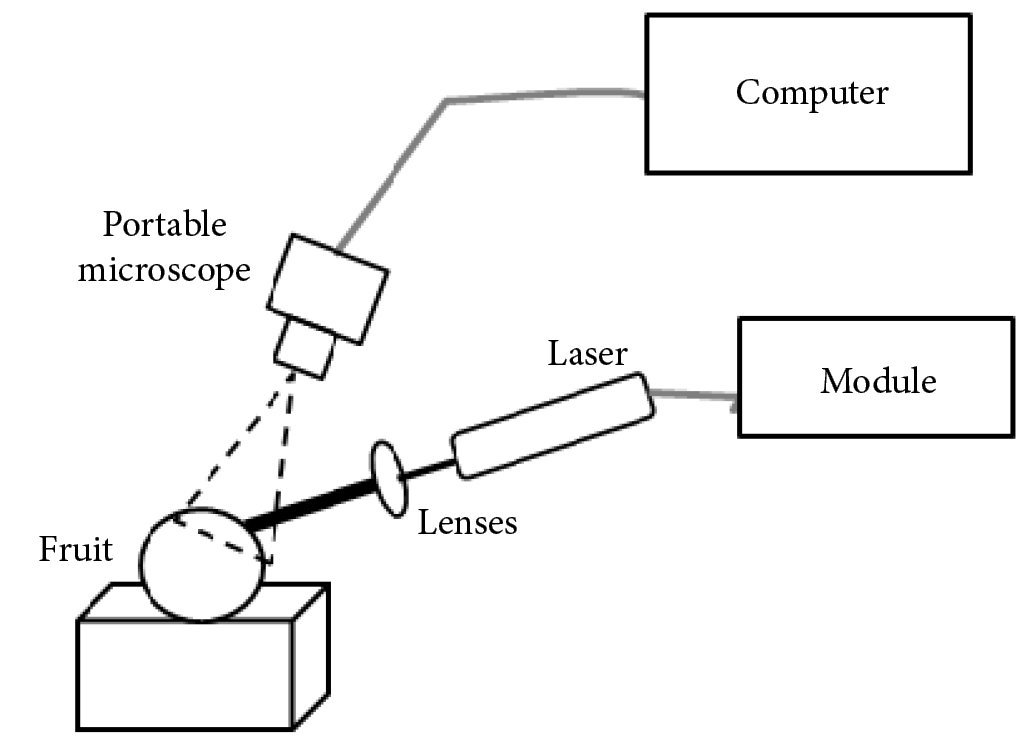
\includegraphics[width=5cm]{figure/materiais/setup.jpg}
\caption{Esquema demostrativo dos materiais utilizados na captura das imagens.}
\label{fig:laser}
\end{figure}


\newpage
\subsection{Statistical analysis}

Para a avaliação da normalidade dos dados foi utilizado o teste de Normalidade Shapiro Wilk (SK) os dados que seguiram a normalidade foi utilizado método de analise de variância de um fator (ANOVA) e o teste de Tukey para comparações multiplas, para os que não seguiram a normalidade foi utilizado Teste de Kruskal-Wallis. As médias, a partir dos dados obtidos , foram submetidas regressão buscando analisar o comportamento sob a perspectiva de progressão do tempo de maturação, foi testado os modelos lineares e polinomial, considerando o melhor ajuste com R2 ≥ 80\%.

\section{Results}

\subsection{Results of the analysis of the moment of inertia}


Os valores de Momento de Inercia capturados pelo método de biospeckle dinâmico apresentaram diferença significativa, valores constantes na Tabela 2. Com relação ao comportamento da regressão, os primeiros níveis demonstraram um comportamento linear.
%tabela para massa

\begin{table}[ht]\footnotesize
\centering
\caption{Análise de Variância com significância a 5\% para perda de Massa Fresca}
\label{anova_massa}
\begin{tabular}{|c|l|l|l|l|l|l|}
\hline
Fonte de variação & SQ       & gl & MQ         & F           & valor P                         \\ \hline
Entre grupos      & 317,5684 & 4  & 79,3921   & 0,556925424 & {\color[HTML]{FD6864} 0,69641138}\\ \hline
Dentro de grupos  & 2851,0855 & 20 & 142,554275 &             &                            \\ \hline
\end{tabular}
\end{table}

% tabela para MI
\begin{table}[ht]\footnotesize
\centering
\caption{Análise de Variância com significância a 5\% para Momento de Inércia}
\label{anova_mi}
\begin{tabular}{|c|l|l|l|l|l|l|}
\hline
Fonte de variação & SQ       & gl & MQ         & F           & valor P                            \\ \hline
Entre grupos      & 245,81444 & 4  & 61,453610
   & 3,127652197
 & {\color[HTML]{FD6864} 0,0376379\\ \hline
Dentro de grupos  & 392,96959 & 20 & 19,64847951
 &             &                            \\ \hline
\end{tabular}
\end{table}
\begin{figure}[h!]  
\centering
\subfigure[ref1][Regressão para perda de massa fresca]{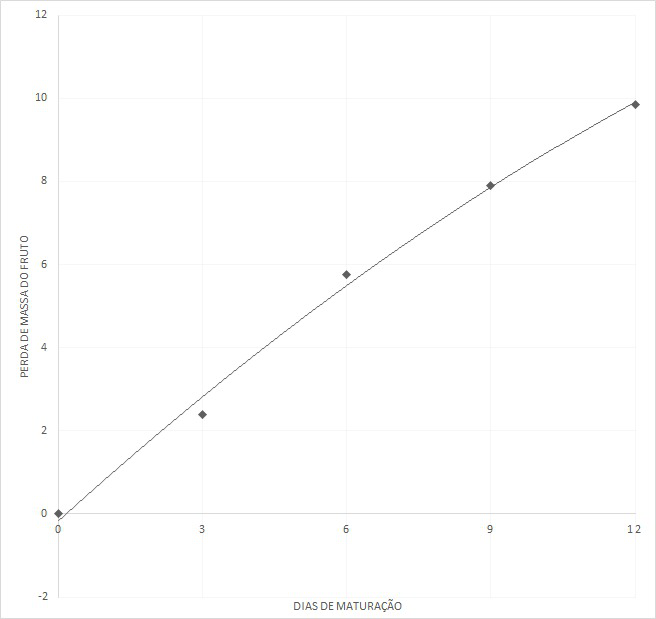
\includegraphics[width=5cm]{figure/estatistica/regressao_massa}}
\qquad
\subfigure[ref2][Regressão para perda de MI]{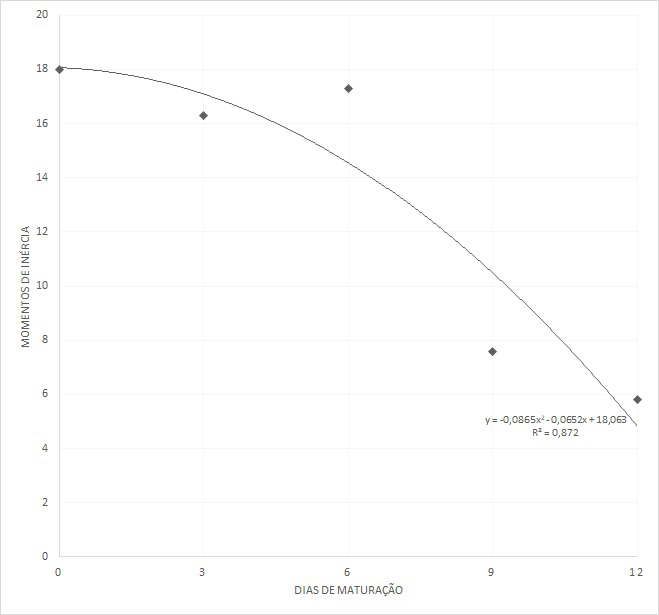
\includegraphics[width=5cm]{figure/estatistica/regressao_inercia}}
\caption{(a) Regressão perda de massa fresca e (b) Regressão MI.}
\label{regressao_MI_massa}
\end{figure}







\newpage

\subsection{Frequency Mapping by Fourier and Wavelets preliminary tests}

Os dados mostram haver correlação entre a perda de massa fresca das amostas e os níveis de atividade monitorados pelo biospeckle laser, conforme pode ser observados nos diferentes níveis. Partido da Figura \ref{atividades1}a à Figura  \ref{atividades5}a, resultantes do processamento com o  método DG  e reconstrução de uma única banda de frequência. Onde nos valores mais altos de massa \ref{atividades1}a e  \ref{atividades2}a apresenta auta atividade representada principalmente pelas cores amarelo e verde de tons mais claros, já as imagens \ref{atividades4} e \ref{atividades5} os tons se apresentam mais baixos, mais próximos dos azul e cinza. O uso de apenas uma banda para o processamento com o DG demonstrou seletividade em diferentes níveis de massa. \citet{Cardoso2011} demostrou haver influência dos diferentes níveis de água em grãos de milho influenciam as taxas de atividades registradas pelo biospeckle onde, o grão com presenças de rachaduras e conseguinte maior evaporação da água apresentou níveis maiores de atividade que os grão que não apresentaram rachaduras, corroborando com este experimento, haja vista que, quanto maior a presença da água no material biológico,  maior os níveis de biospeckle. Utilizando a Analise de Variância (ANOVA) com o teste de Tukey com o nível de significância a 5\%, não ouve diferença significativa  entre os diferentes níveis de massa durante os períodos de maturação, como pode ser observado na figura \ref{regressao_MI_massa} porém, observando o comportamento dos gráficos de dispersão para perda de massa e momento de inércia, podemos verificar uma tendencia %verificar o que colocar aqui.




\begin{figure}[h!]  
\centering
\subfigure[ref1][Diferença Generalizada 0 Dia]{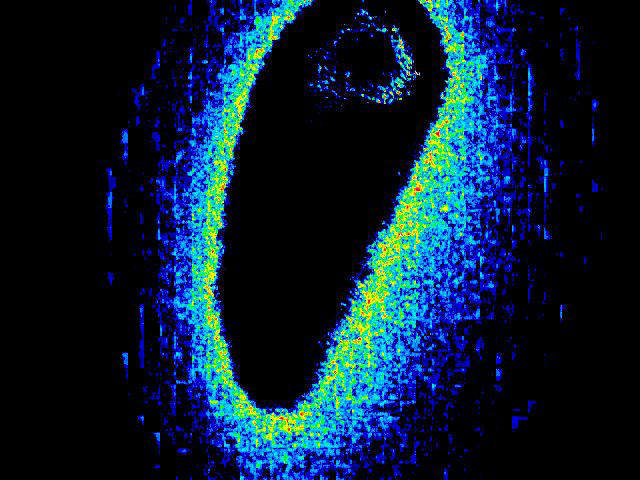
\includegraphics[width=5cm]{figure/dgs/dia_1.png}}
\qquad
\subfigure[ref2][Histograma da amostra]{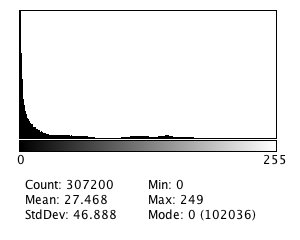
\includegraphics[width=5cm]{figure/histograma/umidade_1.png}}
\caption{(a) Diferença Generalizada e (b) Histograma das amostras primeiro dia.}
\label{atividades1}
\end{figure}

\begin{figure}[h!]
\centering
\subfigure[ref3][Diferença Generalizada]{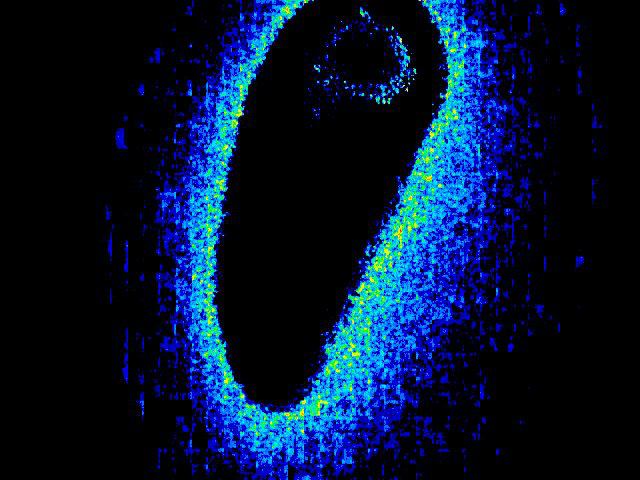
\includegraphics[width=5cm]{figure/dgs/dia_2.png}}
\qquad
\subfigure[ref4][Histograma da amostra]{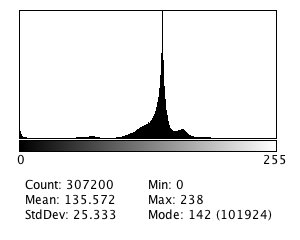
\includegraphics[width=5cm]{figure/histograma/umidade_2.png}}
\caption{(a) Diferença Generalizada e (b) Histograma das amostras segundo dia.}
\label{atividades2}
\end{figure}

\begin{figure}[h!]
\centering
\subfigure[ref5][Diferença Generalizada]{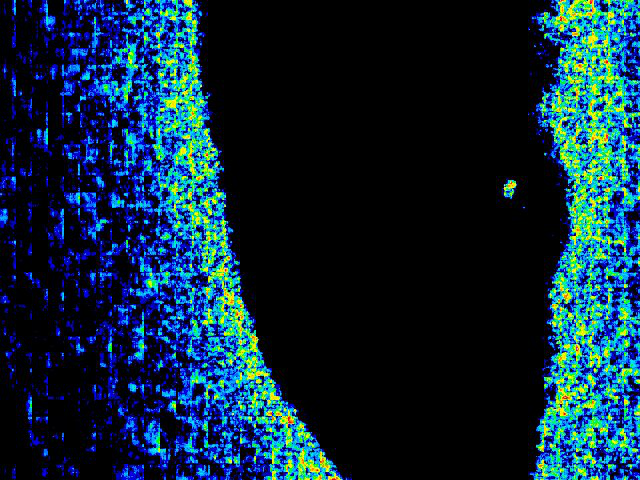
\includegraphics[width=5cm]{figure/dgs/dia_3.png}}
\qquad
\subfigure[ref6][Histograma da amostra]{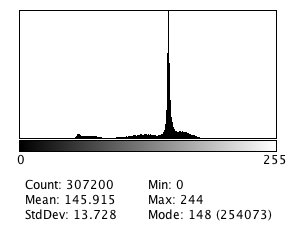
\includegraphics[width=5cm]{figure/histograma/umidade_3.png}}
\caption{(a) Diferença Generalizada e (b) Histograma das amostras terceiro dia.}
\label{atividades3}
\end{figure}

\begin{figure}[h!]
\centering
\subfigure[ref7][Diferença Generalizada]{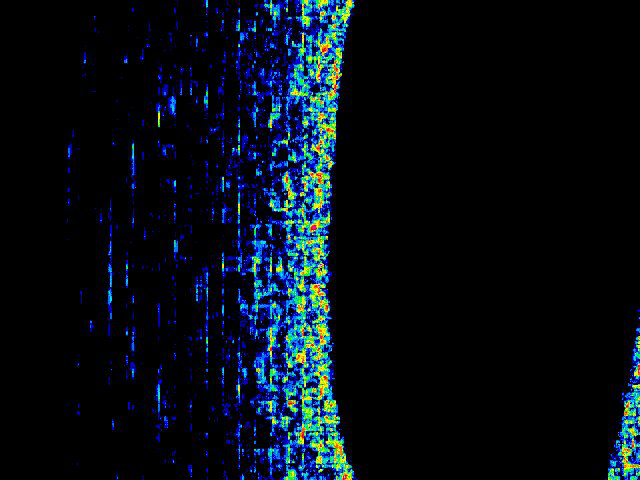
\includegraphics[width=5cm]{figure/dgs/dia_4.png}}
\qquad
\subfigure[ref8][Histograma da amostra]{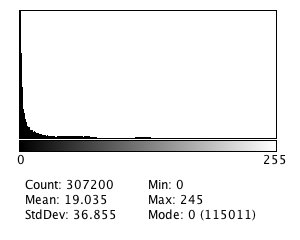
\includegraphics[width=5cm]{figure/histograma/umidade_4.png}}
\qquad
\caption{(a) Diferença Generalizada e (b) Histograma das amostras quarto dia.}
\label{atividades4}
\end{figure}
\begin{figure}[h!]
\centering
\subfigure[ref9][Diferença Generalizada]{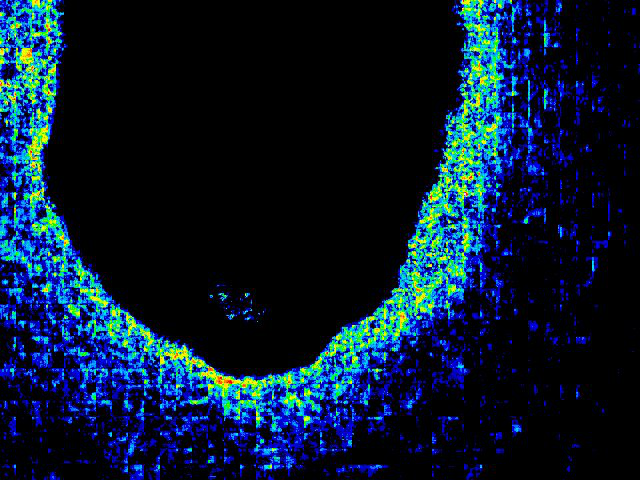
\includegraphics[width=5cm]{figure/dgs/dia_5.png}}
\qquad
\subfigure[ref10][Histograma da amostra]{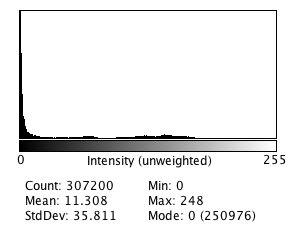
\includegraphics[width=5cm]{figure/histograma/umidade_5.png}}
\label{atividades5}
\end{figure}
\\
\newpage

\section{Conclusion}
Este trabalho apresentou resultados favoráveis ao avaliar não-destrutivamente os níveis de maturação do tomate Caline IPA-06 através do uso de processamento de imagens baseado no biospeckle dinâmico associando-as a métodos rotineiros e numéricos. Tanto para amostragem espectral tendo como base o DG ou amostragem numérica baseado no MI. Descobrimos que o momento de inércia em segunda ordem (MI) é sensível a mudança nos níveis de massa fresca, conforme se perde a quantidade de massa do fruto se reduziu a ocorrência do fenômeno.

\bibliography{mendeley}

\end{document}
